\documentclass[11pt,a4paper]{article}

\usepackage[T1]{fontenc}
\usepackage[utf8]{inputenc}
\usepackage[english]{babel}
\usepackage{lmodern}
\usepackage{amsmath,amssymb,amsfonts}
\usepackage{booktabs}
\usepackage{geometry}
\usepackage{graphicx}
\usepackage{microtype}
\usepackage{enumitem}
\usepackage[numbers,sort&compress]{natbib}
\usepackage{caption}
\usepackage{titlesec}
\usepackage{hyperref}

\geometry{margin=1in}
\hypersetup{
  hidelinks,
  pdftitle={MSc Research Proposal: Coherent and Dissipative Transport in Simple Open Quantum Networks},
  pdfauthor={Pedro Henrique}
}
\setlist[itemize]{leftmargin=1.4em}
\setlist[enumerate]{leftmargin=1.6em}
\renewcommand{\arraystretch}{1.12}
\captionsetup{font=small,labelfont=bf}
\titleformat{\section}{\large\bfseries}{\thesection.}{0.6em}{}
\titleformat{\subsection}{\normalsize\bfseries}{\thesubsection.}{0.5em}{}

\title{\textbf{MSc Research Proposal -- FAMB/FFCLRP-USP}\\
\large Coherent and Dissipative Transport in Simple Open Quantum Networks}

\author{
Pedro Henrique\\
\small Graduate Program in Physics Applied to Medicine and Biology (FAMB)\\
\small Intended supervisor: Prof.\ Dr.\ Alexandre Souto Martinez
}

\date{April 2026}

\begin{document}

\maketitle

\begin{abstract}
This project aims to study transport in small open quantum networks described as
graphs. The main idea is to compare how different graph configurations behave
when coherent hopping competes with local dephasing and capture into a sink. The
goal is to understand, within a simple and controlled model, when coherence
helps transport, when it hinders it, and how different network structures
change that balance. The project will use a tight-binding Hamiltonian in the
single-excitation sector and a Lindblad master equation as the starting
framework. The central comparison will be carried out across a small set of
graph families, using sink efficiency as the main observable and population
dynamics plus coherence as secondary diagnostics. The emphasis is on physical
clarity, systematic comparison between graph structures, and reproducible
numerical results.
\end{abstract}

\noindent\textbf{Keywords:} open quantum systems; quantum transport; graph models;
decoherence; Lindblad dynamics.

\section{Introduction}

Transport in quantum systems can already become nontrivial in very small models.
If one prepares a single excitation in a network of coupled sites, its evolution
depends both on the coherent hopping between sites and on the dissipative action
of the environment. Even in a small graph, these ingredients can generate very
different behaviors: fast transfer, destructive interference, trapping in
inefficient pathways, or suppression of transport by strong decoherence
\citep{mohseni_2008,plenio_huelga_2008,rebentrost_2009,caruso_2009}.

The present proposal studies this problem in a deliberately simple way. The
network will be treated as a graph with a small number of vertices. Different
graph configurations --- such as chains, rings, and complete graphs --- will be
compared under the same basic open-system dynamics. In this way, the project is
not centered on one very specific geometry, but on how geometry itself shapes
the competition between coherent and dissipative transport.

This is a good MSc problem because it is simple enough to be fully understood,
but rich enough to produce nontrivial physics. It also allows a gradual
progression: first understand the minimal model well, then compare different
graph structures, and only later consider more elaborate extensions. The
proposal is therefore centered on the smallest model that can already answer a
real physics question: how topology and dephasing compete to determine
transport toward a target channel in an open quantum network
\citep{breuer_petruccione_2007,rivas_huelga_2012}.

\section{Research question}

The central question of the project is:

\begin{quote}
\emph{How do graph topology, coherent hopping, and local dephasing determine
transport to a sink in simple open quantum networks?}
\end{quote}

More specifically, the project asks:
\begin{itemize}
  \item how transport changes from one graph configuration to another;
  \item whether some graph structures are naturally more robust against
  decoherence than others;
  \item whether intermediate dephasing can improve transport in some cases.
\end{itemize}

\section{Objectives}

\subsection{General objective}

To study coherent and dissipative transport in simple open quantum networks by
comparing different graph configurations within a common minimal model.

\subsection{Specific objectives}

\begin{enumerate}
  \item Implement graph-based models with two to five sites.
  \item Compare at least three graph families: chain, ring, and complete graph.
  \item Describe coherent hopping, local dephasing, and sink capture in a common
  open-system framework.
  \item Use sink efficiency as the main observable for comparing graph
  configurations.
  \item Use population dynamics and coherence as secondary observables for
  interpreting the transport mechanism in each graph.
  \item Determine how transport changes with the dephasing rate and with graph
  structure.
  \item Identify parameter regimes in which dephasing suppresses or enhances
  transport.
\end{enumerate}

\section{Minimal model}

\subsection{Graph representation}

The network will be described as a graph with $N$ vertices. Each vertex
represents a site that can host the excitation, and each edge represents a
coherent hopping channel between two sites. In the single-excitation sector, the
natural basis is $\{|i\rangle\}_{i=1}^{N}$, where $|i\rangle$ denotes the
excitation localized at vertex $i$.

Different graph configurations correspond to different adjacency structures:
\begin{itemize}
  \item in a chain, only nearest neighbors are connected;
  \item in a ring, the chain is closed periodically;
  \item in a complete graph, every site is connected to every other site.
\end{itemize}

This graph viewpoint is central to the project. The aim is not only to solve one
transport model, but to compare how transport changes when the underlying graph
changes.

\subsection{Coherent dynamics}

The coherent part of the model is given by the tight-binding Hamiltonian
\begin{equation}
H = \sum_{i=1}^{N}\epsilon_i |i\rangle\langle i|
  + \sum_{i\neq j} J_{ij}|i\rangle\langle j|.
\label{eq:hamiltonian}
\end{equation}

Here, $\epsilon_i$ are site energies and $J_{ij}$ are hopping amplitudes. The
matrix $J_{ij}$ is directly determined by the graph structure. Therefore, by
changing the graph, one changes the coherent transport pathways available to the
excitation.

\subsection{Open-system dynamics}

The dissipative evolution will be modeled by the Lindblad master equation
\begin{equation}
\frac{d\rho}{dt}
= -i[H,\rho]
+ \sum_k \left(
L_k \rho L_k^\dagger
- \frac{1}{2}\{L_k^\dagger L_k,\rho\}
\right),
\label{eq:lindblad}
\end{equation}
with $\hbar=1$.

This is the simplest standard framework for combining coherent dynamics and
dissipation in a physically controlled way
\citep{breuer_petruccione_2007,rivas_huelga_2012}. It is sufficient for a first
study of the coherent-to-dissipative crossover in small networks.

\subsection{Dissipative channels}

The initial project will use two main dissipative mechanisms.

\paragraph{Local dephasing.}
At each site,
\begin{equation}
L_i^{(\phi)} = \sqrt{\gamma_{\phi,i}}\; |i\rangle\langle i|.
\label{eq:dephasing}
\end{equation}
This channel preserves population but suppresses coherence between different
sites.

\paragraph{Useful sink capture.}
Successful transport will be represented by an absorbing sink state
$|s\rangle$, fed by a chosen target site $|t\rangle$:
\begin{equation}
L^{(\mathrm{sink})} = \sqrt{\kappa}\; |s\rangle\langle t|.
\label{eq:sink}
\end{equation}

The sink is included because the project is not about arbitrary spreading on a
graph, but about transport toward a target channel.

\paragraph{Parasitic loss.}
In the numerical implementation, a separate loss channel is also available:
\begin{equation}
L_i^{(\mathrm{loss})} = \sqrt{\Gamma_i}\; |\ell\rangle\langle i|.
\label{eq:loss}
\end{equation}
This distinction is useful because it separates successful transfer from
irrelevant dissipation. However, in the first stage of the MSc project, the
central emphasis will remain on sink transport and dephasing. The loss channel
can be treated initially as a secondary comparison layer.

\subsection{Main observables}

The main observable of the project will be the sink efficiency at time $T$,
\begin{equation}
\eta(T)=\rho_{ss}(T),
\label{eq:efficiency}
\end{equation}
which measures the probability that the excitation has reached the sink by time
$T$.

This will be the main quantity used to compare different graph configurations.

Two secondary observables will be used to interpret why one graph transports
better than another.

\paragraph{Population dynamics.}
The site populations
\begin{equation}
P_i(t)=\rho_{ii}(t)
\label{eq:population}
\end{equation}
show how the excitation moves across the graph before reaching the sink.

\paragraph{Coherence.}
The site-basis coherence will be monitored through
\begin{equation}
C_{\ell_1}(\rho)=\sum_{i\neq j}|\rho_{ij}|.
\label{eq:coherence}
\end{equation}

Together, sink efficiency, population dynamics, and coherence are sufficient for
the core version of the project. Quantities such as purity and entropy remain
available in the codebase, but they will be treated as optional diagnostics
rather than central observables.

\subsection{Regimes of interest}

The project will compare three physically distinct regimes:
\begin{itemize}
  \item \textbf{Coherent regime:} dephasing is weak compared with the coherent
  hopping scale, so interference strongly affects the transport pathways.
  \item \textbf{Intermediate regime:} dephasing competes with coherent hopping
  without completely destroying coherence. This is the regime in which
  transport enhancement may appear in some graph topologies
  \citep{plenio_huelga_2008,coates_2021,coates_2023,jacob_2024}.
  \item \textbf{Strongly dissipative regime:} dephasing dominates the
  dynamics and tends to suppress coherent transport.
\end{itemize}

This division is useful because it turns the parameter scan into a clear
physical comparison rather than a purely numerical sweep.

\section{Methodology}

\subsection{Step 1: smallest graphs}

The project will begin with the simplest nontrivial graphs, such as two-site and
three-site systems. The goal is to understand in detail how coherent hopping,
sink coupling, and dephasing interact in the most elementary settings.

\subsection{Step 2: comparison between graph families}

The next step will compare chains, rings, and complete graphs with up to five
sites. The goal here is to isolate the role of graph structure. Instead of
treating topology as a secondary detail, the project makes topology itself one
of the main control parameters.

\subsection{Step 3: parameter sweeps}

For each graph family, the dephasing rate will be varied systematically. This
will make it possible to identify:
\begin{itemize}
  \item coherent-dominated regimes;
  \item intermediate regimes in which dephasing changes the transport pattern;
  \item strongly dissipative regimes in which transport is suppressed.
\end{itemize}

\subsection{Step 4: optional extensions}

Once the minimal model is fully understood, simple extensions can be added:
\begin{itemize}
  \item static disorder in the site energies;
  \item explicit comparison between useful sink capture and parasitic loss;
  \item reduced variables for a compact regime map.
\end{itemize}

These will be treated as natural developments, not as mandatory starting points.

\section{Experimental motivation from superconducting circuits}

Although the proposed MSc work is theoretical and computational, it is useful
to keep contact with experimentally relevant platforms. Superconducting circuits
provide such a motivation without changing the minimal structure of the
project. They offer programmable couplings, controlled dissipation, and direct
access to small network geometries, which makes them a natural long-term target
for comparison between simulation and experiment.

This motivation is already supported by the literature. Poto\v{c}nik
\emph{et al.} used superconducting circuits to emulate light-harvesting
transport models \citep{potocnik_2018}. More recently, Zhang \emph{et al.}
reported steady quantum transport in a superconducting processor
\citep{zhang_2024_transport}. In parallel, the open-system description of
superconducting qubits continues to be an active methodological theme
\citep{naeij_2025}. For the present proposal, this literature will be used only
as a short experimental motivation and as a guide for plausible parameter
windows. The core MSc problem remains the study of small graph models
themselves.

\section{Why this project is scientifically useful}

The project becomes more useful if it is treated as a systematic comparison of
graph-based transport models rather than as a collection of isolated numerical
examples. Its scientific value comes from four features:
\begin{enumerate}
  \item it compares different graph structures within the same physical model;
  \item it keeps the model simple enough to be fully understood;
  \item it can identify when decoherence helps or hinders transport;
  \item it can be implemented as a reproducible computational benchmark.
\end{enumerate}

This gives the project a clear path toward a future article: a systematic study
of coherent and dissipative transport across simple graph families, with emphasis
on physical interpretation, regime classification, and reproducibility.

\section{Infrastructure already available}

The project does not start from scratch. The \emph{Quantum-systems} repository
already contains:
\begin{enumerate}
  \item a Lindblad solver,
  \item routines for sink efficiency, population dynamics, coherence, and other
  basic open-system observables,
  \item automated tests,
  \item a one-command transport laboratory that regenerates the main figures,
  metrics, and regime summaries for the proposal,
  \item reproducible conventions for scripts, figures, metrics, and
  configuration files,
  \item a \LaTeX{} pipeline for documentation.
\end{enumerate}

This means that the practical effort can be focused on the physics of the graph
models, rather than on building numerical infrastructure from the ground up.

\section{Preliminary results}

As preparation for this proposal, a first graph-based transport module has
already been implemented in the repository. The current baseline compares three
simple network structures: a complete graph, a disordered ring, and an ordered
chain.

The preliminary results already show that the graph structure matters strongly.
In the complete graph, sink transport improves substantially at an intermediate
dephasing rate. In the ring, the best performance remains near the coherent
limit. In the chain, strong dephasing suppresses transport significantly.

This is exactly the type of behavior that motivates the project: the same
dissipative mechanism can play very different roles depending on the underlying
graph.

\begin{figure}[t]
  \centering
  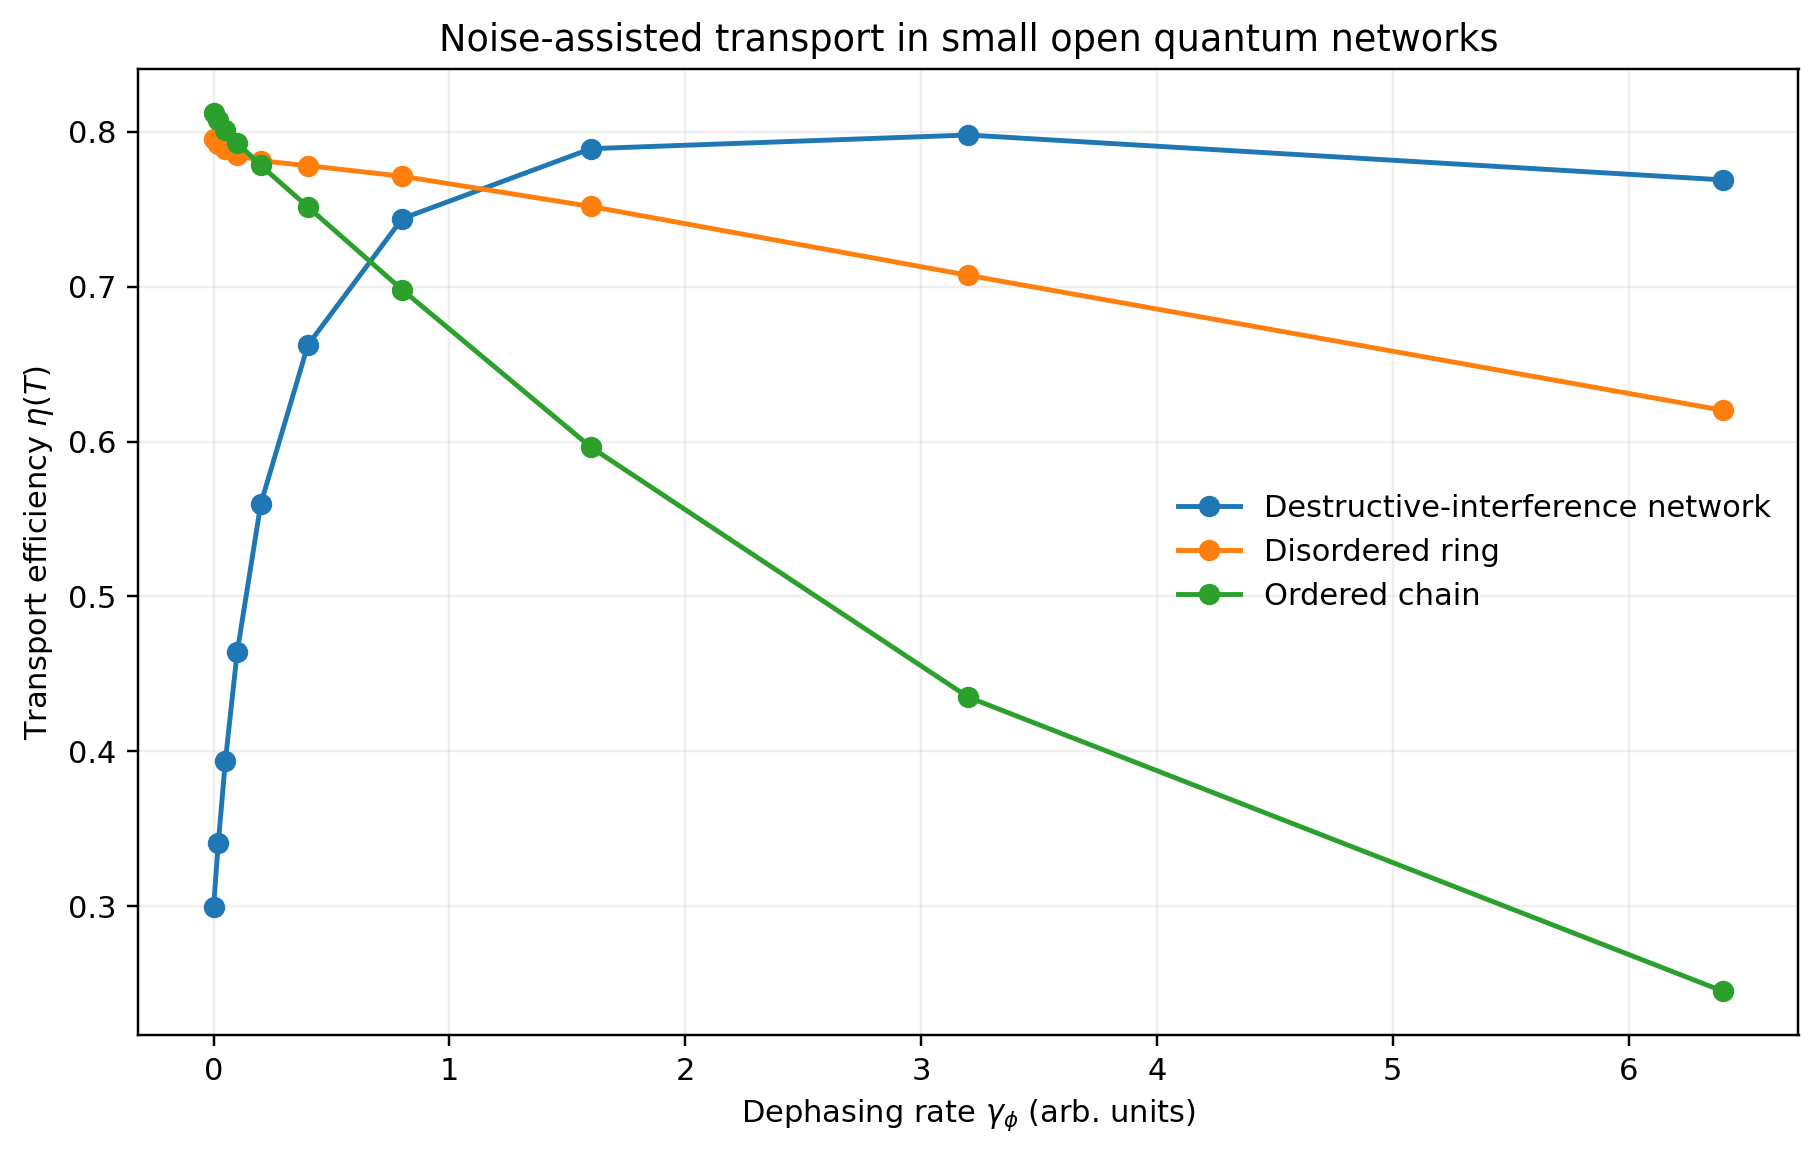
\includegraphics[width=0.92\textwidth]{../../outputs/transport_networks/dephasing_scan/latest/figures/sink_efficiency_by_graph.png}
  \caption{Main comparison figure: sink efficiency $\eta(T)$ as a function of
  the dephasing rate for three graph configurations. This is the principal
  observable of the project because it measures the fraction of excitations
  successfully captured by the sink. The curves already show that the same
  dissipative channel can enhance transport in one topology and suppress it in
  another.}
  \label{fig:efficiency_scan}
\end{figure}

\begin{figure}[t]
  \centering
  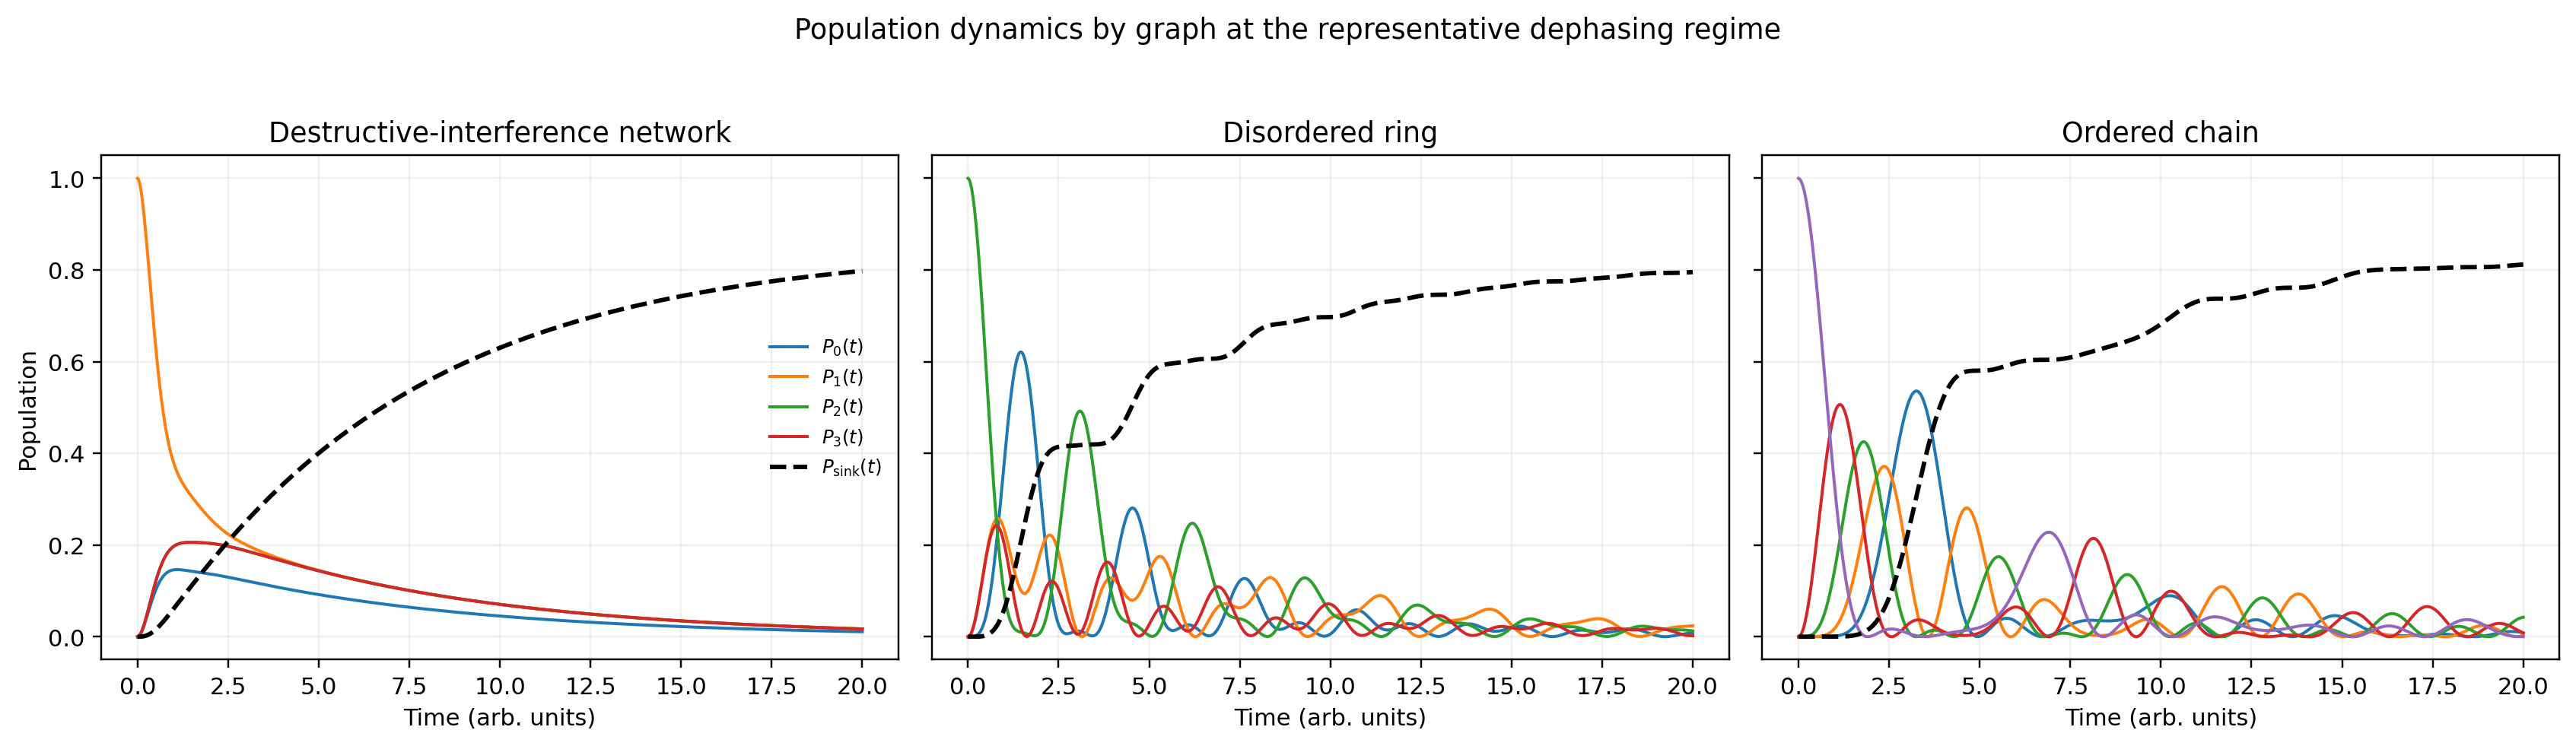
\includegraphics[width=0.96\textwidth]{../../outputs/transport_networks/dephasing_scan/latest/figures/population_dynamics_by_graph.png}
  \caption{Secondary figure: population dynamics in the representative regime
  selected for each graph. The site populations $P_i(t)$ and the sink
  population $P_{\mathrm{sink}}(t)$ show how the excitation propagates through
  the network before capture. This figure is useful for interpreting the
  transport pathways behind the sink-efficiency curves.}
  \label{fig:population_dynamics}
\end{figure}

\begin{figure}[t]
  \centering
  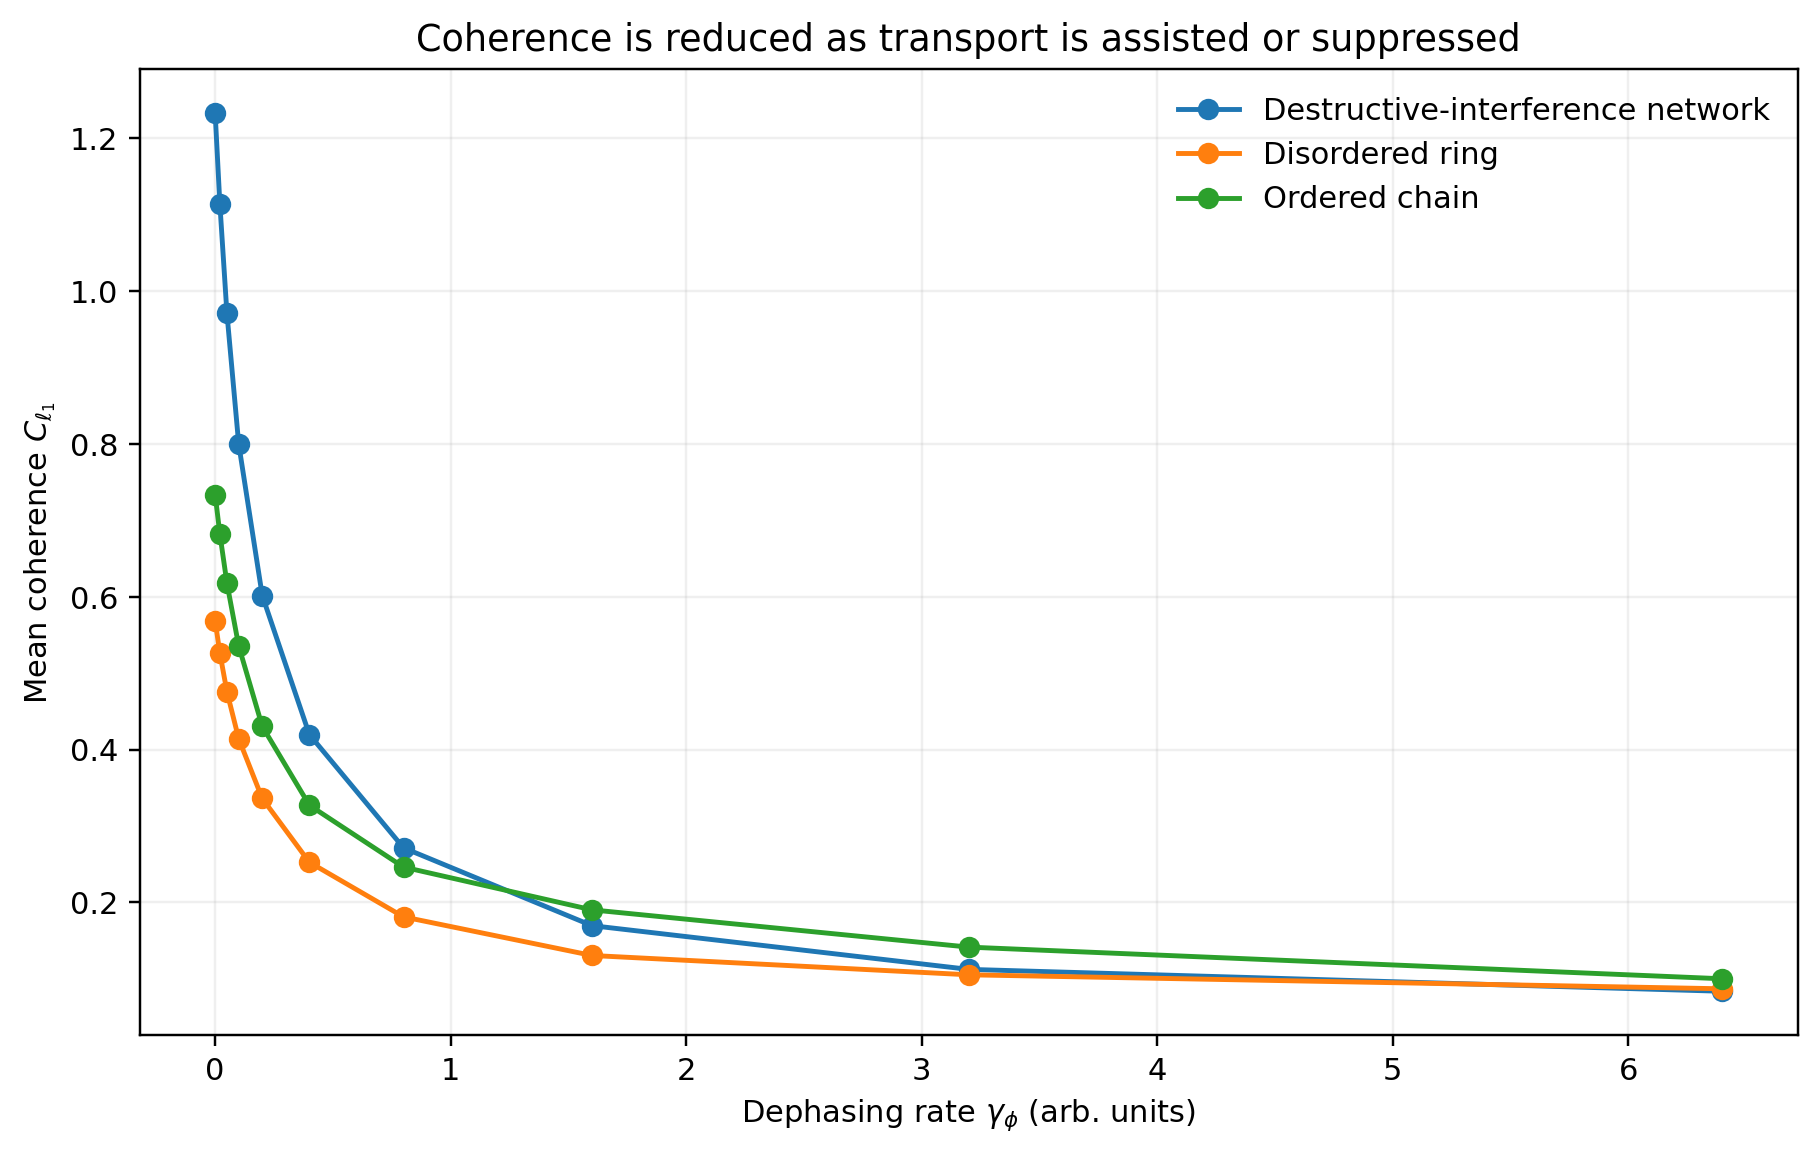
\includegraphics[width=0.92\textwidth]{../../outputs/transport_networks/dephasing_scan/latest/figures/coherence_by_graph.png}
  \caption{Secondary figure: mean coherence $C_{\ell_1}$ as a function of the
  dephasing rate for the same graph configurations. This diagnostic helps
  connect transport performance to the destruction or preservation of quantum
  coherence, without making coherence itself the principal performance metric.}
  \label{fig:coherence_scan}
\end{figure}

\section{Timeline}

The proposed 24-month timeline is:

\begin{center}
\begin{tabular}{p{0.18\textwidth} p{0.72\textwidth}}
\toprule
Period & Main activity \\
\midrule
Months 1--3 & Literature review and full consolidation of the minimal graph
transport model. \\
Months 4--6 & Detailed study of the smallest graphs and simplest topologies. \\
Months 7--9 & Systematic comparison between chains, rings, and complete graphs
under dephasing and sink capture. \\
Months 10--12 & Extended parameter sweeps and interpretation of the coherent-to-
dissipative crossover. \\
Months 13--15 & Optional inclusion of disorder and explicit sink-versus-loss
comparisons. \\
Months 16--18 & Consolidation of the main results and first manuscript draft. \\
Months 19--21 & Dissertation writing. \\
Months 22--24 & Final revision, defense preparation, and reproducibility
cleanup. \\
\bottomrule
\end{tabular}
\end{center}

\section{Expected outcomes}

By the end of the project, the expected outputs are:
\begin{enumerate}
  \item a clear physical account of coherent and dissipative transport in small
  graph-based quantum networks;
  \item a systematic comparison between different graph configurations using
  sink efficiency as the main observable and population dynamics plus coherence
  as secondary diagnostics;
  \item a reproducible computational benchmark with explicit coherent,
  intermediate, and strongly dissipative regimes;
  \item a dissertation and, ideally, a paper based on the graph-comparison
  study.
\end{enumerate}

\section{Conclusion}

This proposal is centered on a simple but physically meaningful problem:
transport in small open quantum networks treated as graphs. Its strength is the
combination of conceptual clarity, systematic topology comparison, and technical
feasibility. That makes it a comfortable and well-structured theme for MSc
supervision, while still leaving room for nontrivial physical results.

\bibliographystyle{unsrtnat}
\bibliography{references}

\end{document}
